\chapter{Method}

We start by deciding on an EEG device to use, then we collect data for both the controlled and organic experiments.

Once data collection is done, we continue with our analysis by training classifiers using various machine learning methods.

\begin{figure}[h]
    \begin{center}
        \includegraphics[width=14cm]{img/method.png}
    \end{center}
    \caption{Overview of the process for the two separate tasks}\label{fig:method}
\end{figure}

The method for our controlled experiment mimics Fucci et al.~\cite{fucci_replication_2019} with some differences (seen in Table~\ref{table:compare-method}): 

\begin{itemize}
        \item We use EEG exclusively.
        \item We used a different device.
        \item We have a smaller \& less diverse sample.
        \item We have reimplemented the task in eeg-notebooks.
        \item We have used the original prose-review images by Floyd et al.~\cite{floyd_decoding_2017}.
\end{itemize}

% Comparing to Fucci and original study
\begin{landscape}
    \rowcolors{4}{gray!25}{white}
\begin{table}
    \begin{center}
        \begin{tabular}{llll}
            \toprule
            \multirow{2}{*}{\textbf{Setting}} & \multicolumn{3}{c}{\textbf{Study}} \\
            \cmidrule(lr){2-4}
            & \makecell[c]{\textbf{This study}} & \makecell[c]{\textbf{Fucci et al.} (2019)} & \makecell[c]{\textbf{Floyd et al.} (2017)} \\
            \midrule
            Experiment site & Lund Univ. (Sweden) & Univ.\ of Bari (Italy) & Univ.\ of Virginia (USA)  \\
            \# Participants & 9 & 28 & 29 \\
            Participants experience & Grads & Undergrads & Grads \& Undergrads \\
            \# Tasks & Variable & 36 tasks & 27 tasks \\
            Task type & \makecell[l]{Code comprehension \\ Prose review} & \makecell[l]{Code comprehension \\ Prose comprehension} & \makecell[l]{Code comprehension \\ Code review \\ Prose review} \\
            Physiological signal & Neural & \Gape[0pt][2pt]{\makecell[l]{Neural \\ Skin \\ Heart}} & Neural \\
            Physiological measure & EEG & \makecell[l]{EEG \\ EDA \\ HR, HRV, BVP} & BOLD \\
            Device & Muse S & \Gape[0pt][2pt]{\makecell[l]{BrainLink Headset \\ Empatica wristband}} & fMRI \\
            Classifier & Riemannian geometry & 8 algorithms & Gaussian Process \\
            Classifier validation & LORO-CV & \Gape[0pt][2pt]{\makecell[l]{LORO-CV \\ Hold-out}} & LORO-CV \\
            Classifier metric & Balanced accuracy (BAC) & Balanced accuracy (BAC) & Balanced accuracy (BAC) \\
            \bottomrule
        \end{tabular}
        \caption{Comparison of this study's method with previous studies.}\label{table:compare-method}
    \end{center}
\end{table}
\rowcolors{2}{}{}

\end{landscape}
\rowcolors{2}{}{}

% Equipment
\section{Devices}
    
    In this section we will briefly describe the different EEG devices we have worked with, and their differences.

    We experimented with several devices but eventually settled on the Muse S. The motivation for choosing the Muse S was mainly due to comfort and ease of use. 

    The other devices considered included the OpenBCI Cyton (with the Ultracortex headset), and the Neurosity Crown.\footnote{Earlier in the work, before we received the Crown, we were also generously gifted a Neurosity Notion DK1 to get a head start.} 

    In our framework, we have implemented support all of the headsets mentioned (and more), such that future work can use whichever device is desired.

    \vspace{0.5cm}
    \begin{table}[H]
    \centering
    \begin{tabular}{llcrr}
        \toprule
        Manufacturer
        & Device
        & Channels
        & Sampling rate
        & Comfort
        \\
        \midrule
        InteraXon
        & Muse S (2020)
        & 4
        & 256Hz
        & High
        \\
        Neurosity
        & Crown (2021)
        & 8
        & 256Hz
        & Medium
        \\
        OpenBCI
        & Cyton (2013) + Ultracortex
        & 8--16
        & 125--250Hz
        & Low
        \\
        \bottomrule
    \end{tabular}
    \caption{Devices used}\label{table:devices}
\end{table}

    \vspace{0.5cm}

    \begin{minipage}{\textwidth}
        \paragraph*{Muse S}
        The Muse S is a 4-channel EEG headband with electrodes at TP9, AF7, AF8, and TP10 (using the modified 10--10 system, seen in Figure~\ref{fig:1010}), with the reference electrode at Fpz~\cite{krigolson_choosing_2017}. Its main advantage is its very comfortable form-factor and long battery life. It's limited by its channel count and electrode placement. It connects using Bluetooth.

        \begin{figure}[H]
            \centering
            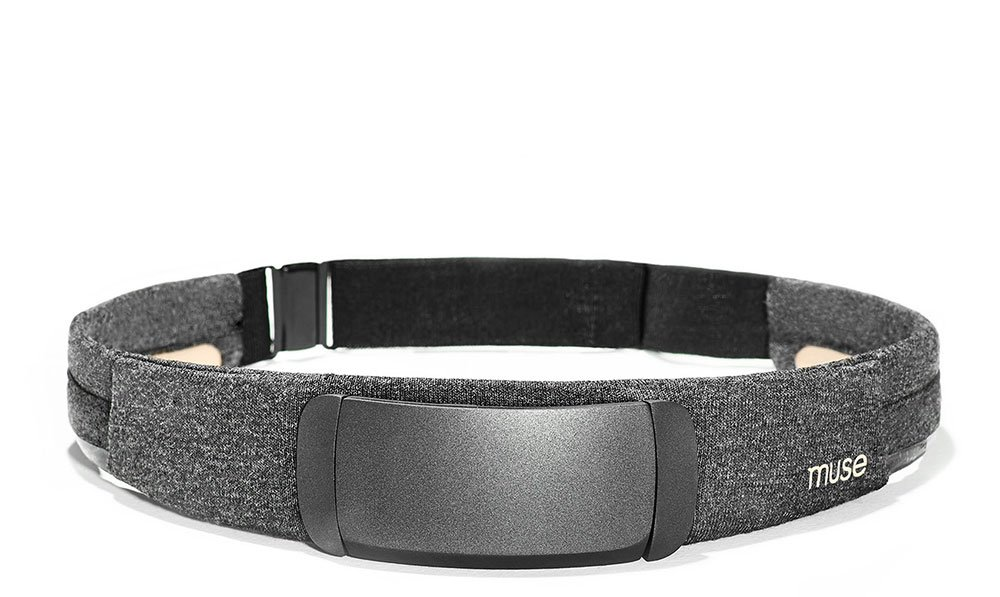
\includegraphics[trim=0 0 0 200,clip,width=100mm]{img/Muse-S.jpg}
            \caption{Muse S}\label{fig:museS}
        \end{figure}
    \end{minipage}

    \begin{minipage}{\textwidth}
        \paragraph*{OpenBCI Cyton}
        The OpenBCI Cyton is a 8-channel EEG board. It is commonly used with the partly 3D-printable OpenBCI Ultracortex Mark IV headset, which allows for flexible electrode placement. OpenBCI also offers an expansion board, the Daisy, which adds 8 additional channels. It connects using Bluetooth.

        %The main disadvantage is the comfort of the Ultracortex headset, which makes it difficult to use for longer sessions. A wet-cap headset would address this, but that has other disadvantages, like being messy and time-consuming.

        \begin{figure}[H]
            \centering
            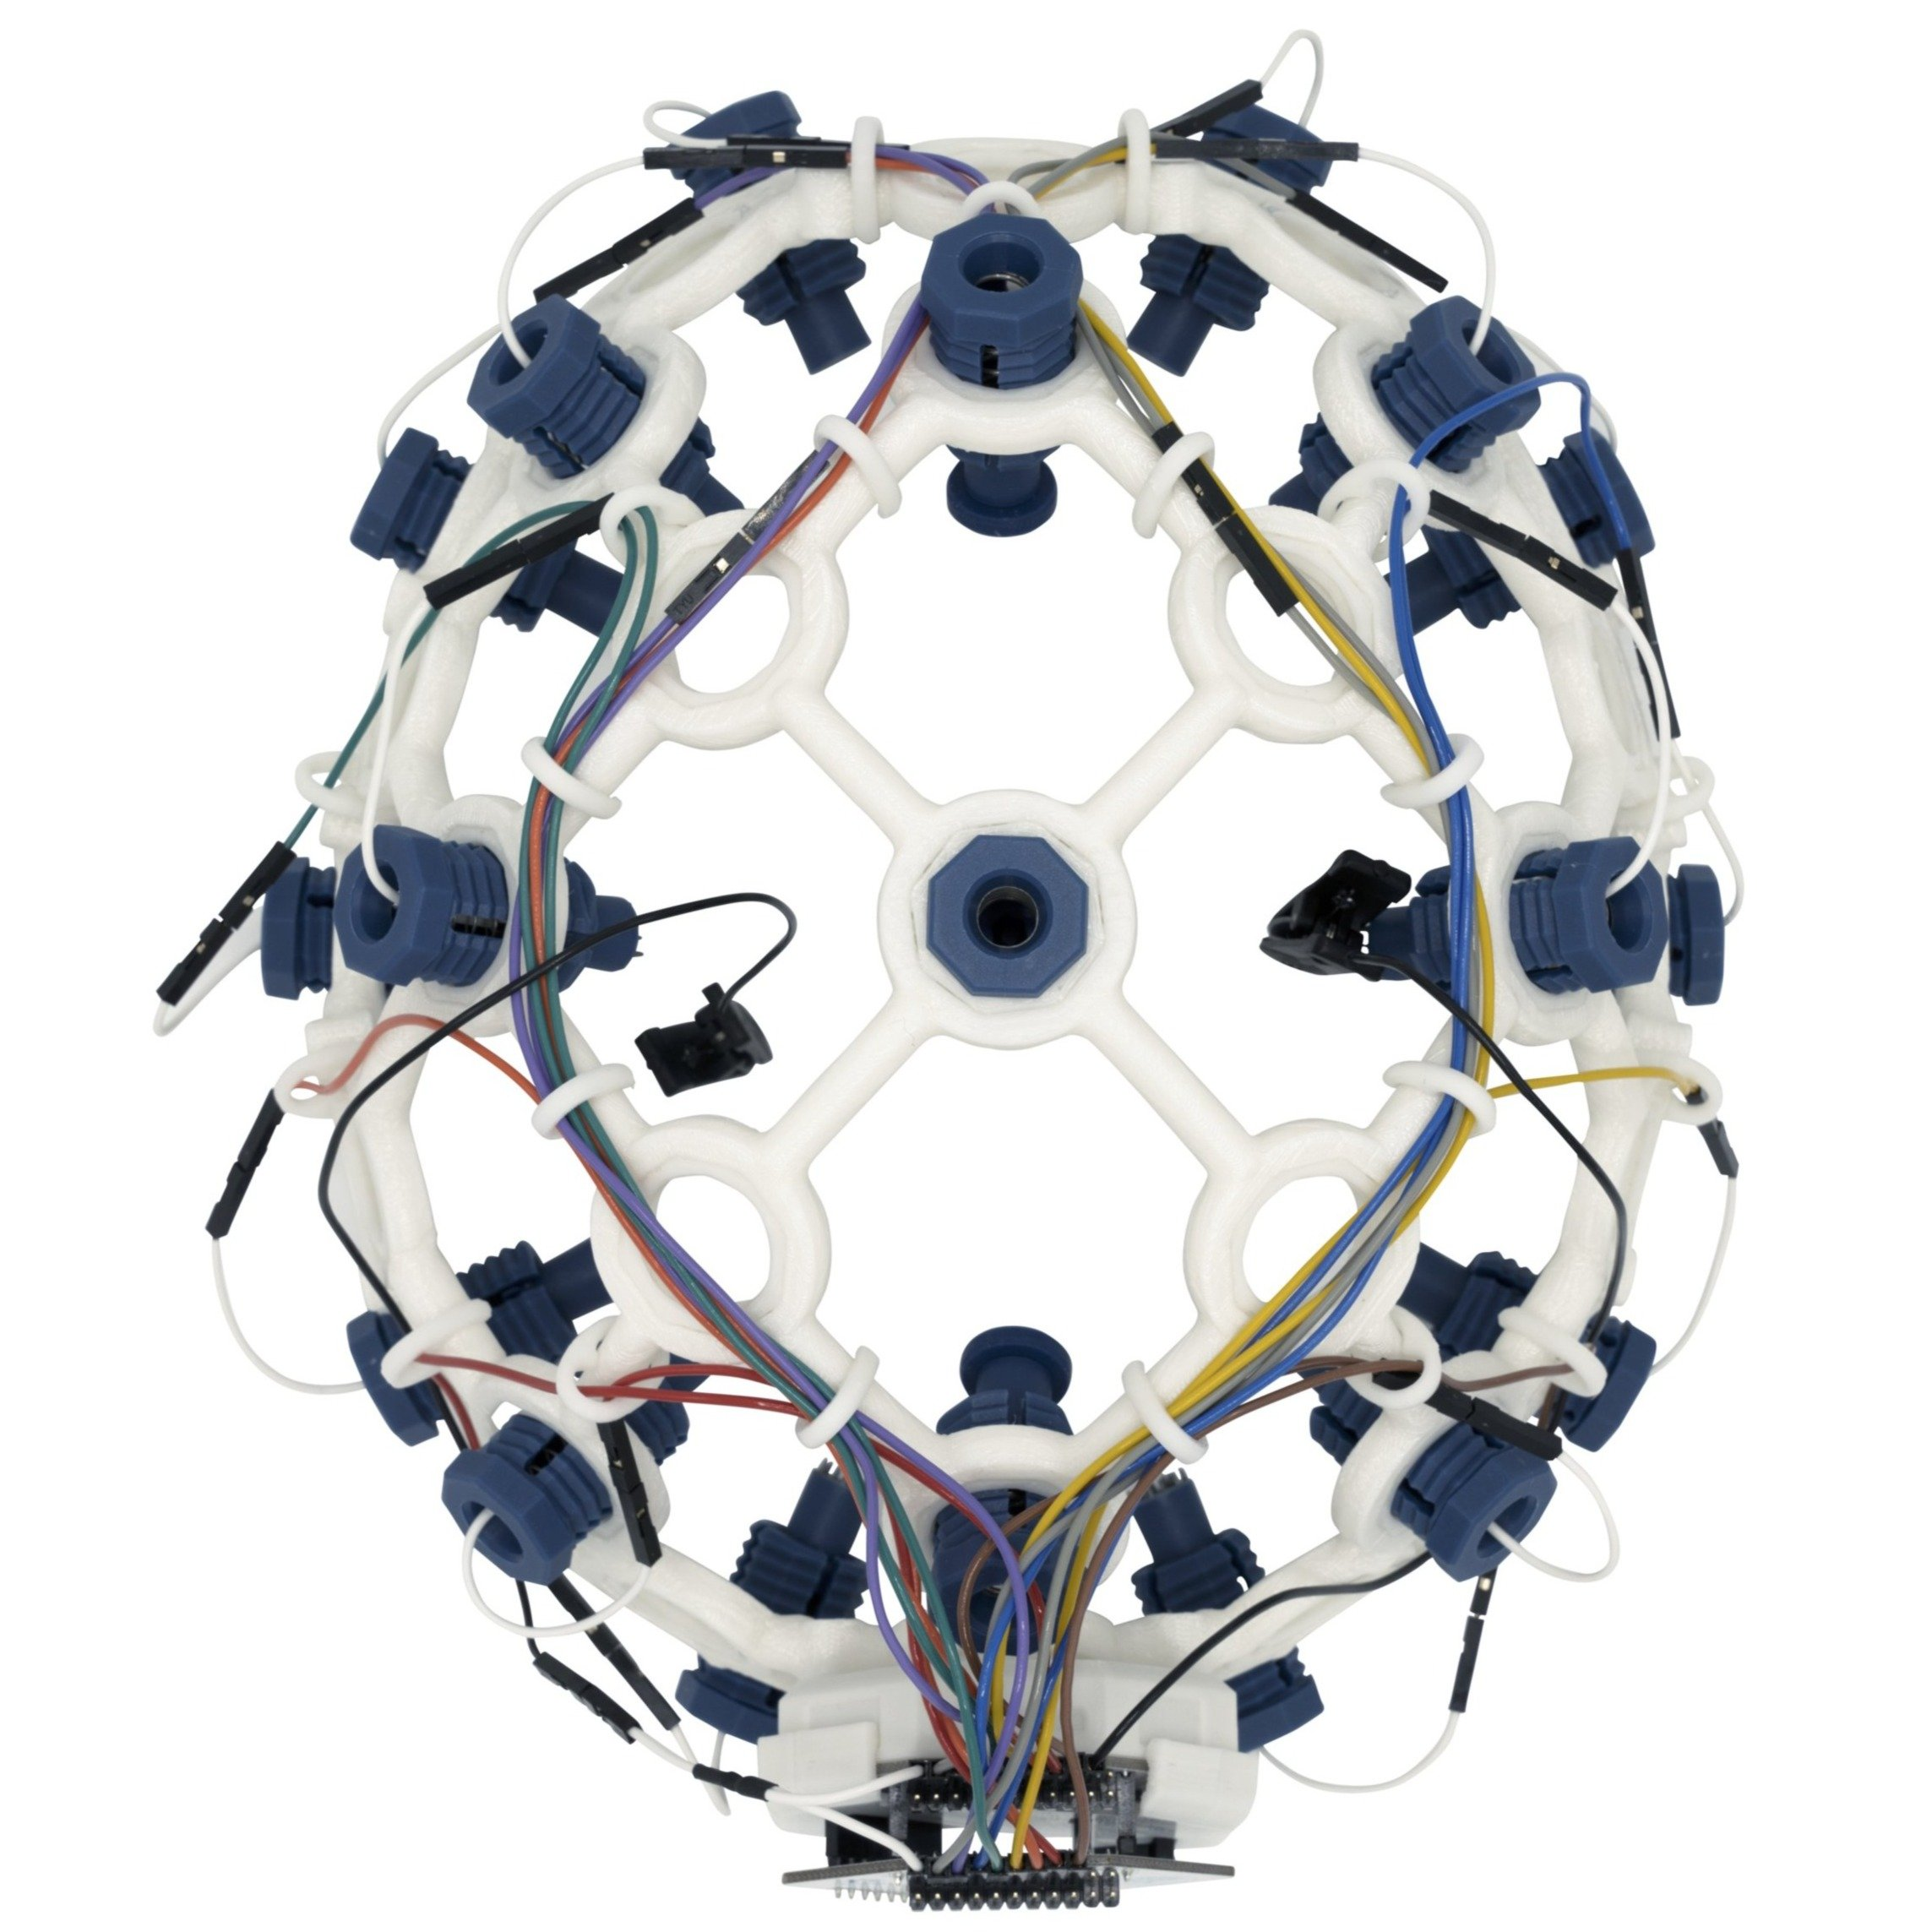
\includegraphics[width=80mm]{img/openbci-cyton.jpg}
            \caption{OpenBCI Cyton + Daisy with Ultracortex Mark IV}\label{fig:cyton}
        \end{figure}
    \end{minipage}

    \vspace{1cm}

    \begin{minipage}{\textwidth}
        \paragraph*{Neurosity Crown}
        The Neurosity Crown is a 8-channel EEG headset. It runs Linux on a quad-core CPU and 1GB RAM, and connects via WiFi. It has electrodes placed at CP3, C3, F5, PO3, PO4, F6, C4, CP4. Reference and bias electrodes at T7 and T8.

        \begin{figure}[H]
            \centering
            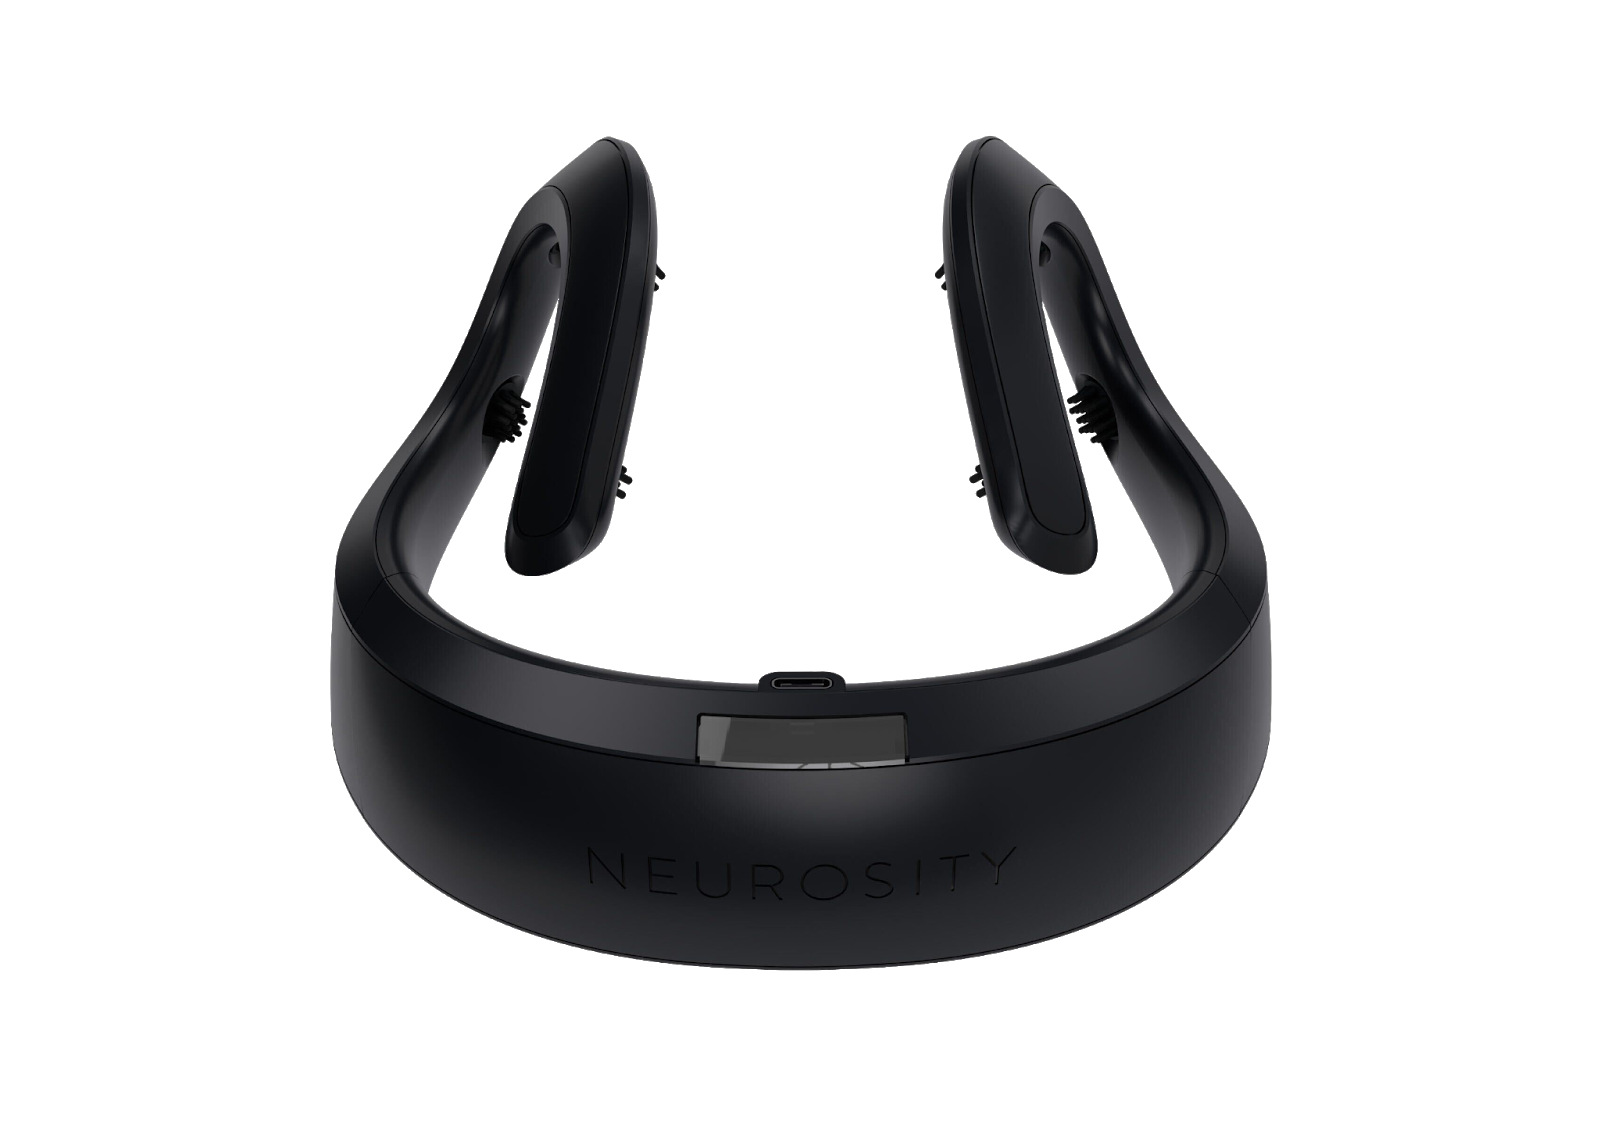
\includegraphics[trim=0 100 0 100,clip,width=100mm]{img/crown-1.png}
            \caption{Neurosity Crown}\label{fig:crown}
        \end{figure}
    \end{minipage}

\pagebreak
\section{Collection}

We need two types of data for the experiments: EEG data, and labels. For the controlled experiment, our labels are whether the stimuli is code or prose. For the organic use experiment, our labels are the device usage categories.

To collect data for the controlled experiment, we:

\begin{enumerate}
    \item Set up the EEG equipment
    \item Use eeg-notebooks to present the stimuli, and record the time markers of when the stimuli changed as labels.
\end{enumerate}

To collect data for the organic use experiment, we:

\begin{enumerate}
    \item Set up the EEG equipment
    \item Configure ActivityWatch to collect device usage data
\end{enumerate}

    \subsection{Collection of EEG data}

        EEG data was collected during organic device use and under controlled conditions. For both conditions, code from the open source \texttt{eeg-notebooks}~\cite{barachant_eeg-notebooks_2020} was adapted to record the raw EEG stream into a CSV file.

        Depending on the device used we require certain software to connect to the devices. We used muse-lsl for the Muse S~\cite{muse-lsl} which in turn uses Lab Streaming Layer. To support OpenBCI and Neurosity devices we used brainflow~\cite{noauthor_brainflow_2020}.

        We have developed `brainwatch', a command-line interface tool, to help us connect to and record from EEG devices. To connect \& record from an EEG device, we can simply run:

        \inputminted{bash}{figures/brainwatch-example.txt}

        We can then check signal quality with: \mintinline{bash}{brainwatch check}

        Or run the following to plot the raw signal: \mintinline{bash}{brainwatch plot}

        Alternatively, we can plot using muse-lsl's built-in plotting functionality: \mintinline{bash}{muselsl view -b Qt5Agg} (seen in Figure~\ref{fig:muselsl-signal}).

        \subsubsection*{During naturalistic device use}\label{section:collect-eeg-naturalistic}

            For the naturalistic device use conditions, we used the Muse S due the superior comfort and ease of use compared with the alternatives, making it especially suitable for long recordings.\footnote{A wet electrode cap system was also considered, but was not used due to being inconvenient to setup.}

            For this experiment we use a single-subject (the experimenter). The subject was asked to go about their usual device activities, often consisting of a mix of work (writing code, writing prose, email) and leisure (watching YouTube, reading Twitter).
            
            We collected approximately 5 hours of EEG data during natural device use, and use the classes defined in Section~\ref{section:collect-usage} as labels for the data.

        \subsubsection*{During code vs prose comprehension task}

            For the controlled condition, we ended up using the Muse S as well due to the comfort and ease of setup.

            We have 9 subjects, sampled by convenience. The subjects were 8 males and one female. Most are in their late 20s or early 30s, except two who are in their 40s.

            The experiment consists of presenting images with code or prose comprehension tasks, seen in Figure~\ref{fig:tasks}. These images are from previous studies on code vs prose comprehension by Floyd et al.~\cite{floyd_decoding_2017} and Fucci et al.~\cite{fucci_replication_2019}. 

            \begin{figure}[H]
                \centering
                \begin{tabular}{cc}
                    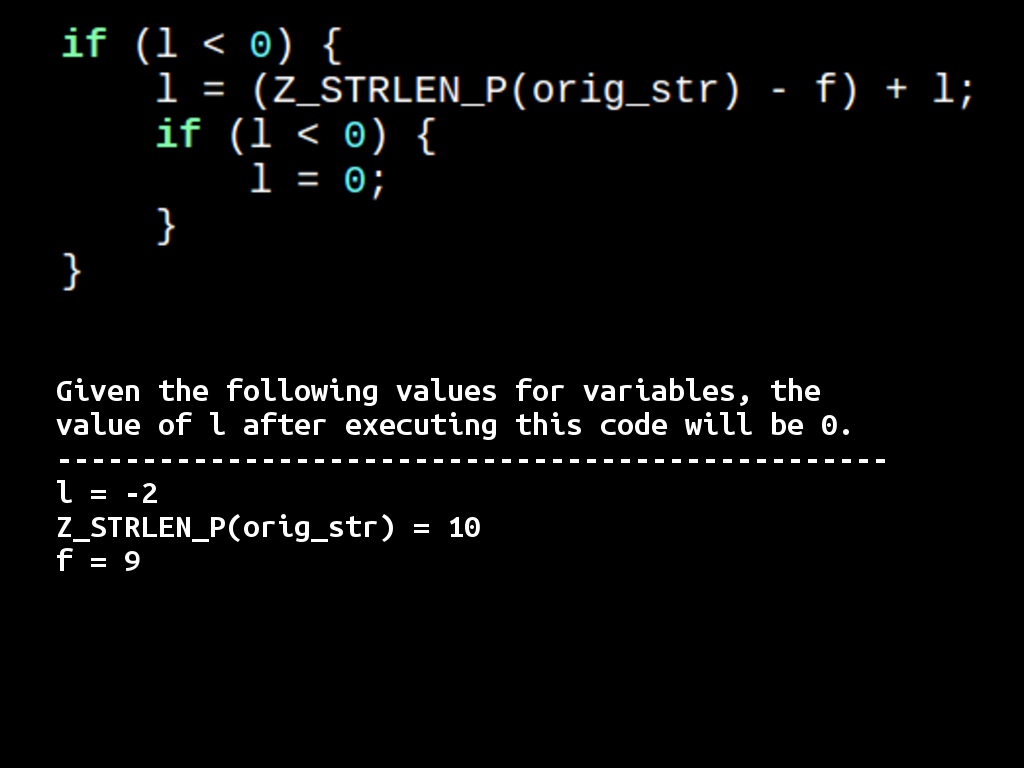
\includegraphics[trim=25 160 0 0,clip,width=75mm]{img/final-1-1.png}
                    &
                    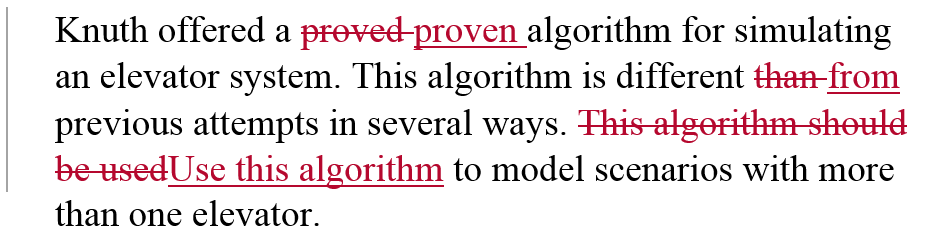
\includegraphics[trim=20 0 20 0,clip,width=75mm]{img/bugs_1.PNG}
                    \\
                    (a) Code comprehension
                    &
                    (b) Prose review
                \end{tabular}
                \caption{Sample of the tasks presented.}\label{fig:tasks}
            \end{figure}

            We note that Fucci et al.~modified the prose comprehension images from the original review-like task to become more comprehension-like, arguably better suited for the task (seen in Figure~\ref{fig:prose-comp-fucci}). However, due to the modified images being in Italian, we have used the original prose review images by Floyd et al.

            \begin{figure}[H]
                \centering
                
\includegraphics[width=90mm]{img/prose-comprehension.png}
                \caption{Sample of the prose comprehension task used by Fucci et al. (translated from Italian).}\label{fig:prose-comp-fucci}
            \end{figure}

            We implemented the task in eeg-notebooks~\cite{barachant_eeg-notebooks_2020}, which uses previously mentioned libraries for data collection as well as PsychoPy~\cite{peirce_psychopy2_2019} to provide the stimuli.

            Before each run, the subject was asked about their gender, age, handedness, and software development experience (specifically experience with C/C++). For good measure, we also asked if the subject had consumed caffeine the hours prior to the experiment.

            After these questions we put the devices on and ensure we get good signal by inspecting it in real time with the viewer provided by muse-lsl (seen in Figure~\ref{fig:muselsl-signal}). The viewer itself does simple bandpass filtering between 3--40Hz, and the signal quality is indicated by the standard deviation of the filtered signal.

            The stimuli images were presented in random order, for all subjects except subject \#1 due to experimenter error (seen in Figure~\ref{fig:timebars}). For each stimuli the subject is asked to answer True/False to the questions posed by the code comprehension stimuli, or Correct/Incorrect for the prose review images. There is a short rest period of 5s between each stimuli. Each experiment run lasted between 10--25 minutes, depending on subject tiredness (subjects were asked to stop when tired).

    \vfill
    \pagebreak
    \subsection{Collection of device activity data}\label{section:collect-usage}

        All device activity is collected using the automated time tracker ActivityWatch~\cite{bjareholt_activitywatch_2020-1}.

        \begin{minipage}{\textwidth}
        ActivityWatch collects data through modules called watchers which report to the ActivityWatch server. It comes with two watchers by default:

        \begin{itemize}
            \item aw-watcher-window, tracks the active window and its title
            \item aw-watcher-afk, tracks if the user is active or not by observing input device activity
        \end{itemize}
        \end{minipage}

        We have also built a custom watcher, aw-watcher-input, to track metrics of mouse and keyboard activity. It tracks by listening to mouse and keyboard events and records the distance in pixels the mouse moves and the number of key presses (but not which key was pressed). Every second this is bundled into an event, the values are reset, and then it continues with the next event. It was inspired by similar functionality in Andrej Karpathy's ulogme~\cite{karpathy_ulogme_2016}.

        A limitation that we have to consider is that the window watcher uses a polling method to track the active window, with a default poll time of 1 second. This means that we can not rely on the timestamps to mark the exact time the window became active/inactive.

        The data from ActivityWatch is processed and categorized such that the resulting data has the 3 columns \mintinline{text}{start, stop, class}. The class is determined by a regular expression that matches on window titles and URLs. For example, the regular expression \mintinline{text}{GitHub|github.com} could be used to match GitHub use.

We chose a few classes for analysis, seen in Table~\ref{table:activity-classes}. Among them we have the classes \emph{Programming} and \emph{Writing}, to see if we can separate these activities in a natural setting.

\begin{table}[h]
    \centering
    \begin{tabular}{ll}
        \toprule
        \textbf{Activity} & \textbf{Regular Expression} \\
        \midrule
        Programming & \texttt{[.](py|rs|js|ts)} \\
        Writing & \texttt{[.](tex|md)} \\
        Twitter & \texttt{Twitter|twitter.com} \\
        YouTube & \texttt{YouTube|youtube.com} \\
        \bottomrule
    \end{tabular}
    \caption{Activity classes used to label EEG data.}\label{table:activity-classes}
\end{table}

\begin{figure}[h]
\begin{minted}{text}
start,               stop,                class
2020-09-20 13:32:51, 2020-09-20 13:34:09, Twitter
2020-09-20 14:44:08, 2020-09-20 14:46:11, YouTube
2020-09-21 09:49:04, 2020-09-21 09:49:35, GitHub->Issues
2020-09-21 09:51:32, 2020-09-21 09:52:23, Programming
2020-09-21 10:20:18, 2020-09-21 10:21:05, Writing
\end{minted}
    \caption{Examples of labeled time windows, collected and categorized with ActivityWatch}\label{code:class-csv}
\end{figure}

\vfill
\pagebreak
\section{Analysis}

    For classification and analysis, we used common open source Python libraries for data analysis, like numpy~\cite{harris2020array}, pandas~\cite{reback2020pandas}, and scikit-learn~\cite{scikit-learn}. In addition, we used less common libraries tailored specifically for working with EEG data, such as MNE~\cite{noauthor_mne-python_2020}, pyriemann~\cite{alexandre_barachant_2020_3715511}, and YASA~\cite{vallat_yasa_2020}.

    \subsection{Labelling}
        When labeling our data we define two levels of granularity: epochs and windows.

        An epoch is a single trial, such as a single stimuli image, which can have variable length due to the experiment setup where the subject decides when to move on to the next stimuli. We label epochs using markers from our experiments.

        A window is a fixed-duration slice of an epoch, such that each window matrix has the same dimensions. This enables us to more easily compute various features which require matrices to be of the same dimension. Windows inherit the label of the epoch from which they belong.

        For the organic device use experiment, we split the EEG data into epochs using the categories assigned by our ActivityWatch script.

        For the controlled experiment, we split the EEG data into epochs using the trial markers, resulting in one epoch per stimuli.

    \subsection{Data transformation}\label{section:transform}

        In order to classify the epochs, which have variable length due to each subject taking a different amount of time to answer each trial, we split each epoch into a fixed-duration window. After some experimentation we found \SI{5}{\second} to be a suitable window size. Once we have our fixed-duration windows, we can use them to train our model and classify new samples.

        Dimensions of each epoch matrix: \[ (n_{\mathrm{samples}}, n_{\mathrm{channels}}) \]

        Where $n_{\mathrm{samples}}$ is the total number of samples for the epoch (variable-length), and $n_{\mathrm{channels}}$ is the number of channels (4 for the Muse S).

        Since the matrix has variable dimensions for each epoch, we split it into \SI{5}{\second} windows, which at the 256Hz sampling frequency of the Muse gives us 1280 samples per window.

        Dimensions of the window matrix: \[ (n_{\mathrm{windows}}, n_{\mathrm{channels}}, 1280) \]

        We experimented with different windowing methods to augment the data, but we ultimately decided against using them, as the methods did not seem to contribute to the performance of trained classifiers.

    \subsection{Data cleaning}

        We reject samples that either:

        \begin{enumerate}
            \item Do not have an assigned class
            \item Have a bad signal quality (as indicated by a signal variance $>40$)
            \item Are too short due to missing samples (such that a 5s window cannot be constructed)
        \end{enumerate}

        The exact number of samples rejected by each cleaning step, as well as the exact parameters used, can be viewed in the code notebooks published alongside this report.

        We also perform bandpass filtering between \SI{3}{\hertz} and \SI{40}{\hertz} to eliminate powerline noise. We can see the results of the bandpass filtering in Figure~\ref{fig:signal-unfiltered} and~\ref{fig:signal-filtered}.

    \subsection{Classification pipelines}

        In this section we describe our classification pipelines which use two different approaches:

        \begin{enumerate}
            \item Use bandpower features to train a common classifier algorithm (such as logistic regression, support vector machines, or random forests).
            \item Use Riemannian methods to work with distances between covariance matrices by using the Riemannian metric, and then apply a common classifier algorithm.
        \end{enumerate}

        \subsubsection{Bandpower-based}

            Bandpower features are simple and commonly used in EEG research for many tasks, including the paper by Fucci et al we seek to improve upon~\cite{fucci_replication_2019}. 

            As a benchmark reference, we implemented classifiers which solely used bandpower features as input, to gain information of how much any improvement from classifier performance is likely due to better EEG equipment versus how much is due to from improved analysis methods.

            To compute this feature, we utilized the bandpower function provided by YASA~\cite{vallat_yasa_2020}. The implementation estimates the power spectral density using Welch's method for each channel, and bins them by their associated frequency band (seen in Table~\ref{table:freq-bands}).

            To further enrich our feature vector, we can use ratios between two frequency bands. As this is what Fucci et al.\ did, we do the same.

            Finally, the pipeline trains 3 models using either logistic regression, support vector machines, or random forests.

        \subsubsection{Riemannian geometry}

            The state of the art in many EEG classification tasks involves the use of Riemannian geometry (described in Section~\ref{section:riemannian-theory}). For this, we used the open source \texttt{pyriemann} library by Alexandre Barachant\footnote{First author of the original paper to apply Riemannian geometry to EEG~\cite{barachant_classification_2013}}.

            Our final pipeline is defined by:

\begin{minted}{python}
from sklearn.pipeline import make_pipeline
from sklearn.linear_model import LogisticRegression
from pyriemann.estimation import Covariances
from pyriemann.spatialfilters import CSP
from pyriemann.tangentspace import TangentSpace

clf = make_pipeline(
    Covariances(),
    CSP(4, log=False),
    TangentSpace(),
    LogisticRegression(),
)
\end{minted}

            We do not perform any hyperparameter optimization.

            \add[inline]{Explanation of pipeline (refer to theory chapter)}

    \begin{comment}
    \subsection{Neural Networks}

        \change[inline]{Future work!}

        One of the classifiers we want to train is a neural network. We use braindecode~\cite{schirrmeister_deep_2017}\cite{noauthor_braindecode_2021}, a neural network library for EEG data that uses PyTorch and integrates it with scikit-learn through skorch.

        The networks provided by braindecode are convolutional\ldots
    \end{comment}

    \subsection{Performance scoring}

        Previous studies have used \emph{balanced accuracy} (BAC) scoring with LORO validation to evaluate model performance. To be able to compare results to previous studies, we do the same. 

        BAC deals with imbalanced datasets by evaluating the performance of the classifier on each class and combining them into a single number. It is defined as the average of recall obtained on each class, or equivalently, the mean of the classifier sensitivity and specificity.

    \subsection{Cross Validation}

        We use \emph{Leave-One-Run-Out} (LORO) cross-validation, a variation of \emph{Leave-One-Group-Out} (LOGO), in order to ensure the samples used in validation are from subjects that are unseen in training. LORO validation generates $n$ folds (one for each subject), with $n-1$ subjects used for training in each fold, and $1$ subject for validation (seen in Table~\ref{table:loro}).

        \definecolor{train}{RGB}{163, 206, 255}
\definecolor{test}{RGB}{255, 181, 84}
\begin{table}[h]
    \centering
    \begin{tabular}{lcccc}
        \toprule
               & Subject 1 & Subject 2 & Subject 3 & Subject 4 \\
        \midrule
        Fold 1 & \cellcolor{test}     & \multicolumn{3}{c}{\cellcolor{train}} \\
        Fold 2 & \cellcolor{train} & \cellcolor{test}     & \multicolumn{2}{c}{\cellcolor{train}     } \\
        Fold 3 & \multicolumn{2}{c}{\cellcolor{train}     } & \cellcolor{test}     & \cellcolor{train} \\
        Fold 4 & \multicolumn{3}{c}{\cellcolor{train}} & \cellcolor{test}     \\
        \bottomrule
    \end{tabular}
    \caption{Example of Leave-One-Run-Out cross validation with 4 subjects. For each fold, subjects marked \textcolor{NavyBlue}{\textbf{blue}} are used for training and subjects marked \textcolor{BurntOrange}{\textbf{orange}} are used for testing.}\label{table:loro}
\end{table}


        % FIXME: Fucci uses the median, should we too?
        To aggregate performance metrics from each fold, we take the median of the performance metrics from each fold (as presented in Section~\ref{section:results}).

        Since we have one run per subject, this LORO cross-validation is effectively an out-of-subject validation, estimating the ability of the classifier to generalize across subjects.

    \begin{comment}
    \subsection{Single subject}

        % TODO: what experiments?
        % TODO: what devices?
        % FIXME: is this out of scope?
        We experimented with single-subject analysis to validate different devices and tasks.
    \end{comment}
